\documentclass[10pt]{article}
\usepackage[french]{babel}
\usepackage[utf8]{inputenc}
\usepackage[T1]{fontenc}
\usepackage{amsmath}
\usepackage{amsfonts}
\usepackage{amssymb}
\usepackage[version=4]{mhchem}
\usepackage{stmaryrd}
\usepackage{graphicx}
\usepackage[export]{adjustbox}
\graphicspath{ {./images/} }
\usepackage{bbold}
\usepackage{caption}
\usepackage{hyperref}
\hypersetup{colorlinks=true, linkcolor=blue, filecolor=magenta, urlcolor=cyan,}
\urlstyle{same}

\begin{document}
\captionsetup{singlelinecheck=false}
\section*{LIMITES DES FONCTIONS}
\section*{Partie 1 : Limite d'une fonction à l'infini}
\section*{1) Limite infinie en $\infty$}
\section*{Définition :}
On dit que la fonction $f$ admet pour limite $+\infty$ en $+\infty$, si $f(x)$ est aussi grand que l'on veut pourvu que $x$ soit suffisamment grand.

Remarque: On a une définition analogue en $-\infty$.

\section*{Exemple:}
La fonction définie par $f(x)=x^{2}$ a pour limite $+\infty$ lorsque $x$ tend vers $+\infty$.\\
On a par exemple : $f(100)=100^{2}=10000$

$$
f(1000)=1000^{2}=1000000
$$

Les valeurs de la fonction deviennent aussi grandes que l'on veut dès que $x$ est suffisamment grand.\\
\includegraphics[max width=\textwidth, center]{0240869f-cc40-4c8d-8725-33efe27b9fb5-01_723_727_913_1178}

\section*{Remarques :}
\begin{itemize}
  \item Une fonction qui tend vers $+\infty$ lorsque $x$ tend vers $+\infty$ n'est pas nécessairement croissante. Par exemple :\\
\includegraphics[max width=\textwidth, center]{0240869f-cc40-4c8d-8725-33efe27b9fb5-01_643_969_1856_552}
  \item Il existe des fonctions qui ne possèdent pas de limite infinie. C'est le cas des fonctions sinusoïdales.\\
\includegraphics[max width=\textwidth, center]{0240869f-cc40-4c8d-8725-33efe27b9fb5-02_460_1027_189_522}
\end{itemize}

\section*{2) Limite finie en $\infty$}
\section*{Définition :}
On dit que la fonction $f$ admet pour limite $\boldsymbol{L}$ en $+\infty$, si $f(x)$ est aussi proche de $L$ que l'on veut, pourvu que $x$ soit suffisamment grand et on note: $\lim _{x \rightarrow+\infty} f(x)=L$.

Remarque : On a une définition analogue en $-\infty$.

\section*{Exemple:}
La fonction définie par $f(x)=2+\frac{1}{x}$ a pour limite 2 lorsque $x$ tend vers $+\infty$. On a par exemple :

$$
\begin{aligned}
& f(100)=2+\frac{1}{100}=2,01 \\
& \begin{aligned}
f(10000) & =2+\frac{1}{10000} \\
& =2,0001
\end{aligned}
\end{aligned}
$$

\begin{center}
\includegraphics[max width=\textwidth]{0240869f-cc40-4c8d-8725-33efe27b9fb5-02_609_1145_1141_776}
\end{center}

Les valeurs de la fonction se resserrent autour de 2 dès que $x$ est suffisamment grand. La courbe de la fonction "se rapproche" de la droite d'équation $y=2$ sans jamais la toucher.

Définition : Si $\lim _{x \rightarrow+\infty} f(x)=L$, la droite d'équation $y=L$ est appelée asymptote horizontale à la courbe de la fonction $f$ en $+\infty$.\\
\includegraphics[max width=\textwidth, center]{0240869f-cc40-4c8d-8725-33efe27b9fb5-02_531_844_2084_616}

\section*{Remarques :}
\begin{itemize}
  \item Lorsque $x$ tend vers $+\infty$, la courbe de la fonction "se rapproche" de son asymptote.
  \item On a une définition analogue en $-\infty$.
\end{itemize}

\section*{3) Limites des fonctions de référence}
\section*{Propriétés :}
\begin{itemize}
  \item $\lim _{x \rightarrow+\infty} x^{2}=+\infty, \lim _{x \rightarrow-\infty} x^{2}=+\infty$
  \item $\lim _{x \rightarrow+\infty} x^{3}=+\infty, \lim _{x \rightarrow-\infty} x^{3}=-\infty$
  \item $\lim _{x \rightarrow+\infty} \sqrt{x}=+\infty$
  \item $\lim _{x \rightarrow+\infty} \frac{1}{x}=0, \lim _{x \rightarrow-\infty} \frac{1}{x}=0$
  \item $\lim _{x \rightarrow+\infty} e^{x}=+\infty, \lim _{x \rightarrow-\infty} e^{x}=0$
\end{itemize}

\section*{Partie 2 : Limite d'une fonction en un réel A}
\section*{1) Définition}
\section*{Définition :}
On dit que la fonction $f$ admet pour limite $+\infty$ en $\boldsymbol{A}$, si $f(x)$ est aussi grand que l'on veut pourvu que $x$ soit suffisamment proche de $A$.

\section*{Exemple :}
La fonction définie par $f(x)=\frac{1}{3-x}+1$ a pour limite $+\infty$ lorsque $x$ tend vers 3 .\\
On a par exemple :\\
$f(2,99)=\frac{1}{3-2,99}+1=101$\\
$f(2,9999)=\frac{1}{3-2,9999}+1=10001$

Les valeurs de la fonction deviennent aussi grandes que l'on veut dès que $x$ est suffisamment proche de 3 .

La courbe de la fonction "se rapproche" de la droite d'équation $x=3$ sans jamais la toucher.\\
\includegraphics[max width=\textwidth, center]{0240869f-cc40-4c8d-8725-33efe27b9fb5-03_1004_785_1625_1109}

Définition : Si : $\lim _{x \rightarrow A} f(x)=+\infty$ ou $\lim _{x \rightarrow A} f(x)=-\infty$, la droite d'équation $x=A$ est appelée asymptote verticale à la courbe de la fonction $f$.\\
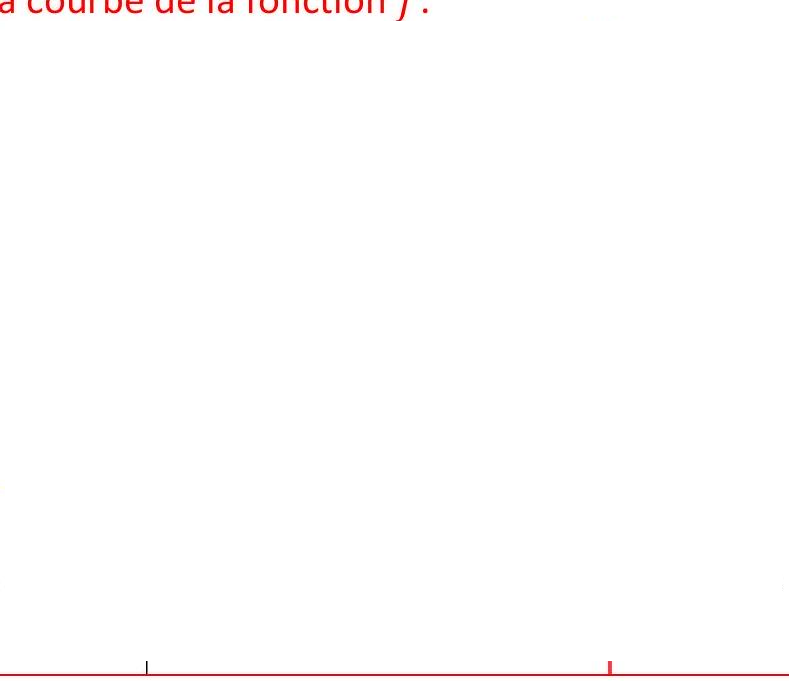
\includegraphics[max width=\textwidth, center]{0240869f-cc40-4c8d-8725-33efe27b9fb5-04_681_789_347_643}\\
2) Limite à gauche, limite à droite :

Exemple :\\
Considérons la fonction inverse définie sur $\mathbb{R}^{*}$ par $f(x)=\frac{1}{x}$.\\
La fonction $f$ admet des limites différentes en 0 selon que :\\
$x>0$ ou $x<0$.

\begin{itemize}
  \item Si $x>0$ : Lorsque $x$ tend vers 0, $f(x)$ tend vers $+\infty$ et on note:\\
$\lim _{\substack{x \rightarrow 0 \\ x>0}} f(x)=+\infty$ ou $\lim _{x \rightarrow 0^{+}} f(x)=+\infty$.\\
On parle de limite à droite de 0
  \item Si $x<0$ : Lorsque $x$ tend vers 0, $f(x)$ tend vers $-\infty$ et on note:\\
$\lim _{\substack{x \rightarrow 0 \\ x<0}} f(x)=-\infty$ ou $\lim _{x \rightarrow 0^{-}} f(x)=-\infty$.\\
On parle de limite à gauche de $\mathbf{0}$.\\
\includegraphics[max width=\textwidth, center]{0240869f-cc40-4c8d-8725-33efe27b9fb5-04_932_746_1192_1125}
\end{itemize}

Méthode : Déterminer graphiquement des limites d'une fonction

\section*{Vidéo https://youtu.be/9nEJCL3s2eU}
On donne ci-dessous la représentation graphique de la fonction $f$.\\
a) Lire graphiquement les limites en $-\infty$, en $+\infty$, en -4 et en 5 .\\
b) Compléter alors le tableau de variations de $f$.

\begin{center}
\begin{tabular}{|c|ccccc|}
\hline
$x$ & $-\infty$ & -4 & 2 & 5 & $+\infty$ \\
\hline
$f(x)$ &  &  &  &  &  \\
\hline
\end{tabular}
\end{center}

\begin{center}
\includegraphics[max width=\textwidth]{0240869f-cc40-4c8d-8725-33efe27b9fb5-05_697_1106_411_484}
\end{center}

\section*{Correction}
a) - $\lim _{x \rightarrow-\infty} f(x)=5 \quad \lim _{x \rightarrow+\infty} f(x)=5$

La courbe de $f$ admet une asymptote horizontale d'équation $y=5$ en $-\infty$ et $+\infty$.

\begin{itemize}
  \item $\lim _{x \rightarrow-4} f(x)=+\infty$
\end{itemize}

La courbe de $f$ admet une asymptote verticale d'équation $x=-4$.

\begin{itemize}
  \item $\lim _{x \rightarrow 5^{-}} f(x)=+\infty$ et $\lim _{x \rightarrow 5^{+}} f(x)=-\infty$
\end{itemize}

La courbe de $f$ admet une asymptote verticale d'équation $x=5$.\\
2)

\begin{center}
\begin{tabular}{|c|cccc||cc|}
\hline
$x$ & $-\infty$ & -4 & 2 & 5 & $+\infty$ &  \\
\hline
 &  & $\nearrow^{+\infty}$ & $\searrow^{+\infty}$ &  & $\searrow_{6}^{+\infty}$ &  \\
$f(x)$ &  &  &  & $\nearrow^{5}$ &  &  \\
 &  &  &  &  &  &  \\
\hline
\end{tabular}
\end{center}

\begin{center}
\includegraphics[max width=\textwidth]{0240869f-cc40-4c8d-8725-33efe27b9fb5-05_654_1061_1998_506}
\end{center}

\section*{Partie 3 : Opérations sur les limites}
\begin{enumerate}
  \item Utiliser les propriétés des opérations sur les limites\\
$\alpha$ peut désigner $+\infty,-\infty$ ou un nombre réel.
\end{enumerate}

\section*{SOMME}
\begin{center}
\begin{tabular}{|l|c|c|c|c|c|c|}
\hline
$\lim _{x \rightarrow \alpha} f(x)=$ & $L$ & $L$ & $L$ & $+\infty$ & $-\infty$ & $+\infty$ \\
\hline
$\lim _{x \rightarrow \alpha} g(x)=$ & $L^{\prime}$ & $+\infty$ & $-\infty$ & $+\infty$ & $-\infty$ & $-\infty$ \\
\hline
$\lim _{x \rightarrow \alpha} f(x)+g(x)=$ & $L+L^{\prime}$ & $+\infty$ & $-\infty$ & $+\infty$ & $-\infty$ & F.I.* \\
\hline
\end{tabular}
\end{center}

\begin{itemize}
  \item Forme indéterminée: On ne peut pas prévoir la limite éventuelle.
\end{itemize}

\begin{table}[h]
\begin{center}
\captionsetup{labelformat=empty}
\caption{PRODUIT $\infty$ désigne $+\infty$ ou $-\infty$}
\begin{tabular}{|l|c|c|c|c|}
\hline
$\lim _{x \rightarrow \alpha} f(x)=$ & $L$ & $L$ & $\infty$ & 0 \\
\hline
$\lim _{x \rightarrow \alpha} g(x)=$ & $L^{\prime}$ & $\infty$ & $\infty$ & $\infty$ \\
\hline
$\lim _{x \rightarrow \alpha} f(x) \times g(x)=$ & $L \times L^{\prime}$ & $\infty$ & $\infty$ & F.I. \\
\hline
\end{tabular}
\end{center}
\end{table}

On applique la règle des signes pour déterminer si le produit est $+\infty$ ou $-\infty$.

\begin{table}[h]
\begin{center}
\captionsetup{labelformat=empty}
\caption{QUOTIENT $\infty$ désigne $+\infty$ ou $-\infty$}
\begin{tabular}{|c|c|c|c|c|c|c|}
\hline
$\lim _{x \rightarrow \alpha} f(x)=$ & $L$ & $L \neq 0$ & $L$ & $\infty$ & $\infty$ & 0 \\
\hline
$\lim _{x \rightarrow \alpha} g(x)=$ & $L^{\prime} \neq 0$ & 0 & $\infty$ & $L$ & $\infty$ & 0 \\
\hline
$\lim _{x \rightarrow \alpha} \frac{f(x)}{g(x)}=$ & $\frac{L}{L^{\prime}}$ & $\infty$ & 0 & $\infty$ & F.I. & F.I. \\
\hline
\end{tabular}
\end{center}
\end{table}

On applique la règle des signes pour déterminer si le quotient est $+\infty$ ou $-\infty$.

Méthode: Calculer la limite d'une fonction à l'aide des formules d'opération

\section*{Vidéo https://youtu.be/at6pFx-Umfs}
Déterminer les limites suivantes :\\
a) $\lim _{x \rightarrow-\infty}(x-5)\left(3+x^{2}\right)$\\
b) $\lim _{x \rightarrow 3^{-}} \frac{1-2 x}{x-3}$

\section*{Correction}
a) $\lim _{x \rightarrow-\infty}(x-5)\left(3+x^{2}\right)=$ ?\\
$\left\{\begin{array}{l}\lim _{x \rightarrow-\infty} x-5=-\infty \\ \lim _{x \rightarrow-\infty} x^{2}=+\infty \text { donc } \lim _{x \rightarrow-\infty} 3+x^{2}=+\infty\end{array}\right.$\\
Comme limite d'un produit : $\lim _{x \rightarrow-\infty}(x-5)\left(3+x^{2}\right)=-\infty$\\
b) $\lim _{x \rightarrow 3^{-}} \frac{1-2 x}{x-3}=$ ?\\
$\left\{\begin{array}{l}\lim _{x \rightarrow 3^{-}} 1-2 x=1-2 \times 3=-5 \\ \lim _{x \rightarrow 3^{-}} x-3=0^{-}\end{array}\right.$\\
Une limite de la forme « $\frac{5}{0}$ » est égale à « $\infty$ ».\\
Donc, d'après la règle des signes, une limite de la forme « $\frac{-5}{0^{-}}$» est égale à « $+\infty$ ».\\
D'où, comme limite d'un quotient: $\lim _{x \rightarrow 3^{-}} \frac{1-2 x}{x-3}=+\infty$.

\section*{2) Cas des formes indéterminée (non exigible)}
Comme pour les suites, on rappelle que :

Les quatre formes indéterminées sont, par abus d'écriture :

$$
\infty-\infty \quad 0 \times \infty \quad \frac{\infty}{\infty} \quad \frac{0}{0}
$$

Méthode : Lever une forme indéterminée à l'aide de factorisations (1) - NON EXIGIBLE

\section*{Vidéo https://youtu.be/4NQbGdXThrk}
Calculer : $\lim _{x \rightarrow+\infty}-3 x^{3}+2 x^{2}-6 x+1$

\section*{Correction}
$\lim _{x \rightarrow+\infty}-3 x^{3}+2 x^{2}-6 x+1=?$

\begin{itemize}
  \item $\left\{\begin{array}{l}\lim _{x \rightarrow+\infty}-3 x^{3}=-\infty \\ \lim _{x \rightarrow+\infty} 2 x^{2}=+\infty .\end{array}\right.$
\end{itemize}

On reconnait une forme indéterminée du type " $\infty-\infty$ ".

\begin{itemize}
  \item Levons l'indétermination en factorisant par le monôme de plus haut degré:
\end{itemize}

$$
-3 x^{3}+2 x^{2}-6 x+1=x^{3}\left(-3+\frac{2}{x}-\frac{6}{x^{2}}+\frac{1}{x^{3}}\right)
$$

\begin{itemize}
  \item $\lim _{x \rightarrow+\infty} \frac{2}{x}=\lim _{x \rightarrow+\infty} \frac{6}{x^{2}}=\lim _{x \rightarrow+\infty} \frac{1}{x^{3}}=0$.
\end{itemize}

Donc, par limite d'une somme :

$$
\lim _{x \rightarrow+\infty}-3+\frac{2}{x}-\frac{6}{x^{2}}+\frac{1}{x^{3}}=-3
$$

\begin{itemize}
  \item $\left\{\begin{array}{l}\lim _{x \rightarrow+\infty}-3+\frac{2}{x}-\frac{6}{x^{2}}+\frac{1}{x^{3}}=-3 \\ \lim _{x \rightarrow+\infty} x^{3}=+\infty\end{array}\right.$
\end{itemize}

Donc, par limite d'un produit :

$$
\lim _{x \rightarrow+\infty} x^{3}\left(-3+\frac{2}{x}-\frac{6}{x^{2}}+\frac{1}{x^{3}}\right)=-\infty
$$

Soit : $\lim _{x \rightarrow+\infty}-3 x^{3}+2 x^{2}-6 x+1=-\infty$.

\section*{Méthode : Lever une forme indéterminée à l'aide de factorisations - NON EXIGIBLE}
Vidéo \href{https://youtu.be/8tAVa4itblc}{https://youtu.be/8tAVa4itblc}\\
Vidéo \href{https://youtu.be/pmWPfsQaRWI}{https://youtu.be/pmWPfsQaRWI}

Calculer :\\
a) $\lim _{x \rightarrow+\infty} \frac{2 x^{2}-5 x+1}{6 x^{2}-5}$\\
b) $\lim _{x \rightarrow-\infty} \frac{3 x^{2}+2}{4 x-1}$

\section*{Correction}
a) - En appliquant la méthode précédente pour le numérateur et le dénominateur cela conduirait à une forme indéterminée du type " $\frac{\infty}{\infty}$ ".

\begin{itemize}
  \item Levons l'indétermination en factorisant les monômes de plus haut degré :
\end{itemize}

$$
\frac{2 x^{2}-5 x+1}{6 x^{2}-5}=\frac{x^{2}}{x^{2}} \times \frac{2-\frac{5}{x}+\frac{1}{x^{2}}}{6-\frac{5}{x^{2}}}=\frac{2-\frac{5}{x}+\frac{1}{x^{2}}}{6-\frac{5}{x^{2}}}
$$

\begin{itemize}
  \item $\lim _{x \rightarrow+\infty} \frac{5}{x}=\lim _{x \rightarrow+\infty} \frac{1}{x^{2}}=\lim _{x \rightarrow+\infty} \frac{5}{x^{2}}=0$.
\end{itemize}

Donc, comme limite de sommes :

$$
\lim _{x \rightarrow+\infty} 2-\frac{5}{x}+\frac{1}{x^{2}}=2 \quad \text { et } \quad \lim _{x \rightarrow+\infty} 6-\frac{5}{x^{2}}=6
$$

\begin{itemize}
  \item Donc, comme limite d'un quotient :
\end{itemize}

$$
\lim _{x \rightarrow+\infty} \frac{2-\frac{5}{x}+\frac{1}{x^{2}}}{6-\frac{5}{x^{2}}}=\frac{2}{6}=\frac{1}{3}
$$

Soit : $\lim _{x \rightarrow+\infty} \frac{2 x^{2}-5 x+1}{6 x^{2}-5}=\frac{1}{3}$.\\
b) - Il s'agit d'une forme indéterminée du type " $\frac{\infty}{\infty}$ ".

\begin{itemize}
  \item Levons l'indétermination en factorisant les monômes de plus haut degré :
\end{itemize}

$$
\frac{3 x^{2}+2}{4 x-1}=\frac{x^{2}}{x} \times \frac{3+\frac{2}{x^{2}}}{4-\frac{1}{x}}=x \times \frac{3+\frac{2}{x^{2}}}{4-\frac{1}{x}}
$$

\begin{itemize}
  \item $\lim _{x \rightarrow-\infty} \frac{1}{x}=\lim _{x \rightarrow-\infty} \frac{2}{x^{2}}=0$
\end{itemize}

Donc, comme limite de sommes :

$$
\lim _{x \rightarrow-\infty} 3+\frac{2}{x^{2}}=3 \quad \text { et } \quad \lim _{x \rightarrow-\infty} 4-\frac{1}{x}=4
$$

\begin{itemize}
  \item Donc, comme limite d'un quotient :
\end{itemize}

$$
\lim _{x \rightarrow-\infty} \frac{3+\frac{2}{x^{2}}}{4-\frac{1}{x}}=\frac{3}{4}
$$

\begin{itemize}
  \item De plus, $\lim _{x \rightarrow-\infty} x=-\infty$, donc, comme limite d'un produit :
\end{itemize}

$$
\lim _{x \rightarrow-\infty} x \times \frac{3+\frac{2}{x^{2}}}{4-\frac{1}{x}}=-\infty
$$

Soit : $\lim _{x \rightarrow-\infty} \frac{3 x^{2}+2}{4 x-1}=-\infty$.

\section*{Méthode : Déterminer une asymptote}
Vidéo \href{https://youtu.be/OLDGK-QkL80}{https://youtu.be/OLDGK-QkL80}\\
Vidéo \href{https://youtu.be/pXDhrx-nMto}{https://youtu.be/pXDhrx-nMto}\\
Soit $f$ la fonction définie sur $\mathbb{R} \backslash\{1\}$ par $f(x)=\frac{-2}{1-x}$.\\
Démontrer que la courbe représentative de la fonction $f$ admet des asymptotes dont on précisera la nature et les équations.

\section*{Correction}
\begin{itemize}
  \item $\lim _{x \rightarrow+\infty} 1-x=-\infty$ donc comme limite d'un quotient, on a : $\lim _{x \rightarrow+\infty} \frac{-2}{1-x}=0$.
\end{itemize}

On prouve de même que : $\lim _{x \rightarrow-\infty} \frac{-2}{1-x}=0$.\\
On en déduit que la droite d'équation $y=0$ est asymptote horizontale à la courbe représentative de $f$ en $+\infty$ et en $-\infty$.

\begin{itemize}
  \item $\lim _{x \rightarrow 1^{-}} 1-x=0^{+}$donc comme limite d'un quotient, on a : $\lim _{x \rightarrow 1^{-}} \frac{-2}{1-x}=-\infty$
\end{itemize}

Et $\lim _{x \rightarrow 1^{+}} 1-x=0^{-}$donc comme limite d'un quotient, on a : $\lim _{x \rightarrow 1^{+}} \frac{-2}{1-x}=+\infty$\\
On en déduit que la droite d'équation $x=1$ est asymptote verticale à la courbe représentative de $f$.\\
\includegraphics[max width=\textwidth, center]{0240869f-cc40-4c8d-8725-33efe27b9fb5-09_869_1049_1835_696}

\section*{Partie 4 : Calculs de limites par composition et comparaison}
\section*{1) Composition de limites}
\section*{Méthode : Déterminer la limite d'une fonction composée}
Vidéo \href{https://youtu.be/DNU1M3li76k}{https://youtu.be/DNU1M3li76k}\\
Vidéo \href{https://youtu.be/f5i}{https://youtu.be/f5i} u8XVMfc\\
Soit la fonction $f$ définie sur $\left[\frac{1}{2} ;+\infty\left[\operatorname{par}: f(x)=\sqrt{2-\frac{1}{x}}\right.\right.$\\
Calculer la limite de la fonction $f$ en $+\infty$.

\section*{Correction}
On a : $\lim _{x \rightarrow+\infty} \frac{1}{x}=0$, donc $\lim _{x \rightarrow+\infty} 2-\frac{1}{x}=2$\\
Donc, comme limite d'une fonction composée : $\lim _{x \rightarrow+\infty} \sqrt{2-\frac{1}{x}}=\sqrt{2}$\\
En effet, si $x \rightarrow+\infty$, on a : $X=2-\frac{1}{x} \rightarrow 2$ et donc : $\lim _{X \rightarrow 2} \sqrt{X}=\sqrt{2}$.

\section*{2) Comparaison}
\section*{Méthode : Calculer une limite par comparaison}
\section*{Vidéo https://youtu.be/OAtkpYMdu7Y}
Calculer : $\lim _{x \rightarrow+\infty} x+\sin x$

\section*{Correction}
\begin{itemize}
  \item $\lim _{x \rightarrow+\infty} \sin x$ n'existe pas.
\end{itemize}

Donc sous la forme donnée, la limite cherchée est indéterminée.

Levons l'indétermination :\\
$\bullet-1 \leq \sin x$, donc : $x-1 \leq x+\sin x$.

\begin{itemize}
  \item Or $\lim _{x \rightarrow+\infty} x-1=+\infty$, donc par comparaison :
\end{itemize}

$$
\lim _{x \rightarrow+\infty} x+\sin x=+\infty
$$

Par abus de langage, on pourrait dire que la fonction $x \longmapsto x-1$ pousse la fonction $x \longmapsto x+\sin x$ vers $+\infty$ pour des valeurs de $x$ suffisamment grandes.

\section*{(c) Copyright}

\end{document}